\documentclass[titlepage, fleqn, a4paper, 12pt, twoside]{article}
\usepackage{geometry}
\usepackage{exsheets} %question and solution environments
\usepackage{amsmath, amssymb, amsthm} %standard AMS packages
\usepackage[utf8]{inputenc}
\usepackage{esint} %integral signs
\usepackage{marginnote} %marginnotes
\usepackage{gensymb} %miscellaneous symbols
\usepackage{commath} %differential symbols
\usepackage{xcolor} %colours
\usepackage{cancel} %cancelling terms
\usepackage[free-standing-units,space-before-unit]{siunitx} %formatting units
	\sisetup
	{
		per-mode=fraction,
		fraction-function=\frac
	}
\usepackage{tikz, pgfplots} %diagrams
	\usetikzlibrary{calc, hobby, patterns, intersections, angles, quotes, spy}
\usepackage{graphicx} %inserting graphics
\usepackage{hyperref} %hyperlinks
\usepackage{datetime} %date and time
\usepackage{enumerate, enumitem} %numbered lists
\usepackage{float} %inserting floats
\usepackage[american voltages]{circuitikz} %circuit diagrams
\usepackage{setspace} %double spacing
\usepackage{microtype} %micro-typography
\usepackage{listings} %formatting code
	\lstset{language=Matlab}
	\lstdefinestyle{standardMatlab}
	{
		belowcaptionskip=1\baselineskip,
		breaklines=true,
		frame=L,
		xleftmargin=\parindent,
		language=C,
		showstringspaces=false,
		basicstyle=\footnotesize\ttfamily,
		keywordstyle=\bfseries\color{green!40!black},
		commentstyle=\itshape\color{purple!40!black},
		identifierstyle=\color{blue},
		stringstyle=\color{orange},
	}
\usepackage{algpseudocode} %algorithms
\usepackage{algorithm} %algorithms
\usepackage{chemfig}
\usepackage{booktabs}
\usepackage{multirow}
\usepackage{todonotes}
\usepackage[noabbrev,capitalize]{cleveref}
\usepackage[section]{placeins}

\newcommand\numberthis{\addtocounter{equation}{1}\tag{\theequation}} %adds numbers to specific equations in non-numbered list of equations

\theoremstyle{definition}
\newtheorem{example}{Example}
\newtheorem{definition}{Definition}

\theoremstyle{theorem}
\newtheorem{theorem}{Theorem}
\newtheorem{law}{Law}

\makeatletter
\@addtoreset{section}{part} %resets section numbers in new part
\makeatother

\newcommand\blfootnote[1]{%
	\begingroup
	\renewcommand\thefootnote{}\footnote{#1}%
	\addtocounter{footnote}{-1}%
	\endgroup
}

\renewcommand{\marginfont}{\scriptsize \color{blue}}

\renewcommand{\tilde}{\widetilde}

\SetupExSheets{solution/print = true} %prints all solutions by default

%opening
\title{Electronic Devices}
\author{Aakash Jog}
\date{2015-16}

\begin{document}

\pagenumbering{roman}
\begin{titlepage}
\newgeometry{margin=0cm}
\maketitle
\end{titlepage}
\restoregeometry
%\setlength{\mathindent}{0pt}

\blfootnote
{	
	\begin{figure}[H]
		
\includegraphics[height = 12pt]{cc.pdf}
		
\includegraphics[height = 12pt]{by.pdf}
		
\includegraphics[height = 12pt]{nc.pdf}
		
\includegraphics[height = 12pt]{sa.pdf}
	\end{figure}
	This work is licensed under the Creative Commons Attribution-NonCommercial-ShareAlike 4.0 International License. To view a copy of this license, visit \url{http://creativecommons.org/licenses/by-nc-sa/4.0/}.
} %CC-BY-NC-SA license

\tableofcontents

\clearpage
\listoffigures

\clearpage
\section{Lecturer Information}

\textbf{Tammy Ben-Yaacov}\\
~\\
E-mail: \href{mailto:tammybenyaacov@gmail.com}{tammybenyaacov@gmail.com}\\

\section{Instructor Information}

\textbf{Asia Shapira}\\
~\\
E-mail: \href{asiasapi@gmail.com}{asiasapi@gmail.com}

\section{Required Reading}

\begin{enumerate}
	\item Streetman, B. Solid State Electronic Devices
\end{enumerate}

\section{Additional Reading}

\begin{enumerate}
	\item Bar-Lev, A. Semiconductor and Electronic Devices
	\item S. M. Sze, Physics of Semiconductor Devices
	\item Kittel, C. (2005). Introduction to Solid State Physics
\end{enumerate}

\clearpage
\pagenumbering{arabic}

\part{}

\section{Energy Bands in Semiconductors}

\begin{figure}[h]
	\centering
	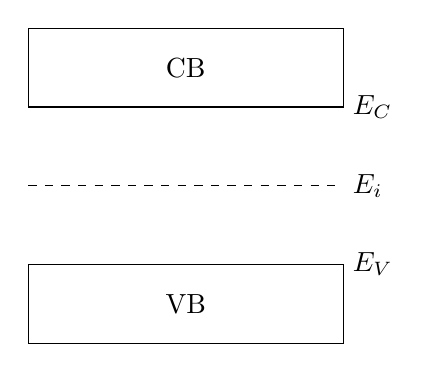
\begin{tikzpicture}
		\def\l{4};
		\def\eConduction{4};
		\def\eValence{2};
		\def\eIntrinsic{{\eConduction * 0.5 + \eValence * 0.5}};

		\begin{scope}
			\draw (0,\eValence) rectangle ++(\l,-1);
			\node at ($ (\l/2,\eValence) + (0,-0.5) $) {VB};
			\node [right] at (\l,\eValence) {$E_V$};
		\end{scope}

		\begin{scope}
			\draw (0,\eConduction) rectangle ++(\l,1);
			\node at ($ (\l/2,\eConduction) + (0,0.5) $) {CB};
			\node [right] at (\l,\eConduction) {$E_C$};
		\end{scope}

		\begin{scope}
			\draw [dashed] (0,\eIntrinsic) -- (\l,\eIntrinsic) node [right] {$E_i$};
		\end{scope}
	\end{tikzpicture}
	\caption{Energy Bands and Intrinsic Energy Level}
	\label{fig:Energy_Bands_and_Intrinsic_Energy_Level}
\end{figure}

\section{Determining Factors for Number of Charge Carriers in Energy Bands}

\subsection{Density of Allowed States in Bands}

The number of allowed states in the conduction and valence bands are denoted as $g_C(E)$ and $g_V(E)$, respectively.\\
There are no allowed states in the gap between the conduction and valence bands.

\begin{theorem}
	\begin{align*}
		g_C(E) & \approx \sqrt{E - E_C}
	\end{align*}
\end{theorem}

\subsection{Probability of Occupancy of Allowed States}

\begin{definition}[Fermi function]
	The probability that an available energy state $E$ will be occupied is
	\begin{align*}
		f(E) & = f_{\text{FD}}(E) \\
                     & = \frac{1}{1 + e^{\frac{E - E_f}{k T}}}
	\end{align*}
	where $E_f$ is the Fermi level or the Fermi energy, and $T$ is the temperature.
\end{definition}
Therefore, the graph of $f(E)$ with respect to $E$ is as in \cref{fig:Graph_of_Fermi_function_for_$T_1_>_T_2_>_T_3$}.
\begin{figure}[h]
	\centering
	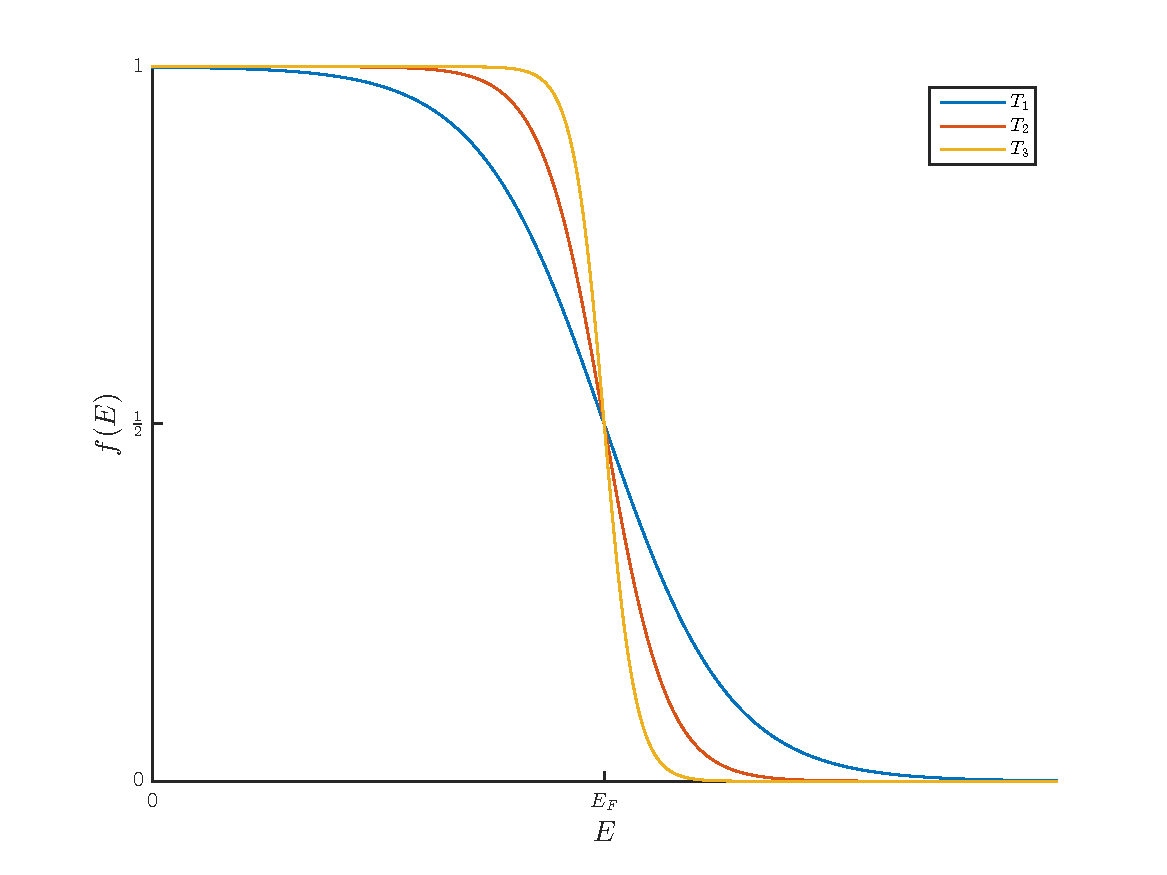
\includegraphics[width = 0.8\textwidth]{./Plots/fermi_function.pdf}
	\caption{Graph of Fermi function for $T_1 > T_2 > T_3$}
	\label{fig:Graph_of_Fermi_function_for_$T_1_>_T_2_>_T_3$}
\end{figure}
If $E < E_f$,
\begin{align*}
	\lim\limits_{T \to 0} f(E) & = 1
\end{align*}
If $E = E_f$,
\begin{align*}
	f(E) & = \frac{1}{2}
\end{align*}
If $E_f < E$,
\begin{align*}
	\lim\limits_{T \to 0} f(E) & = 0
\end{align*}
Therefore, at $0 \kelvin$, $f(E)$ is the unit step function.
Therefore, at $0 \kelvin$, all electrons are at available energy levels less than $E_f$, i.e. in the valence band.
Hence, the conduction band is empty.

\section{Number of Electrons in Conduction Band}

\begin{theorem}
	Electrons in semiconductors obey Fermi-Dirac statistics.
\end{theorem}

Consider an energy band of thickness $\dif E$, at energy $E$, in the conduction band.
Therefore, the number of electrons in the band is
\begin{align*}
	\dif n(E) & = g_C(E) f(E) \dif E
\end{align*}
Therefore, the total number of electrons in the conduction band are
\begin{align*}
	n & = \int\limits_{E_C}^{E_{C} + \Delta} g_C(E) f(E) \dif E
\end{align*}
where $\Delta$ is the thickness of the conduction band.\\
As there are no allowed states above the conduction band,
\begin{align*}
	n & = \int\limits_{E_C}^{\infty} g_C(E) f(E) \dif E
\end{align*}

\section{Position of $E_F$}

The graphs of $f(E)$ and $1 - f(E)$ are as in \cref{fig:Graph_of_$f(E)$_and_$1_-_f(E)$} and ???.
\begin{figure}[h]
	\centering
	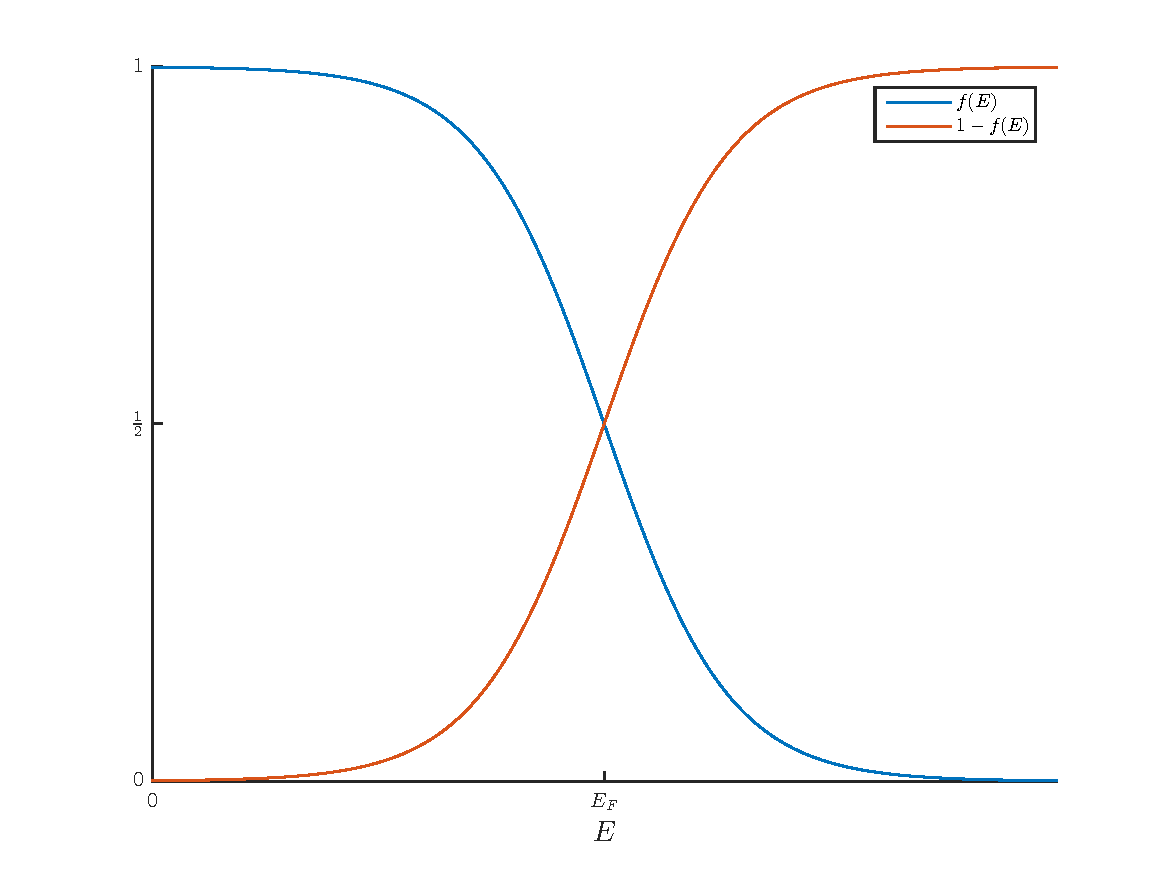
\includegraphics[width = 0.8\textwidth]{./Plots/fermi_function_and_one_minus_fermi_function.pdf}
	\caption{Graph of $f(E)$ and $1 - f(E)$}
	\label{fig:Graph_of_$f(E)$_and_$1_-_f(E)$}
\end{figure}
\begin{figure}[h]
	\centering
	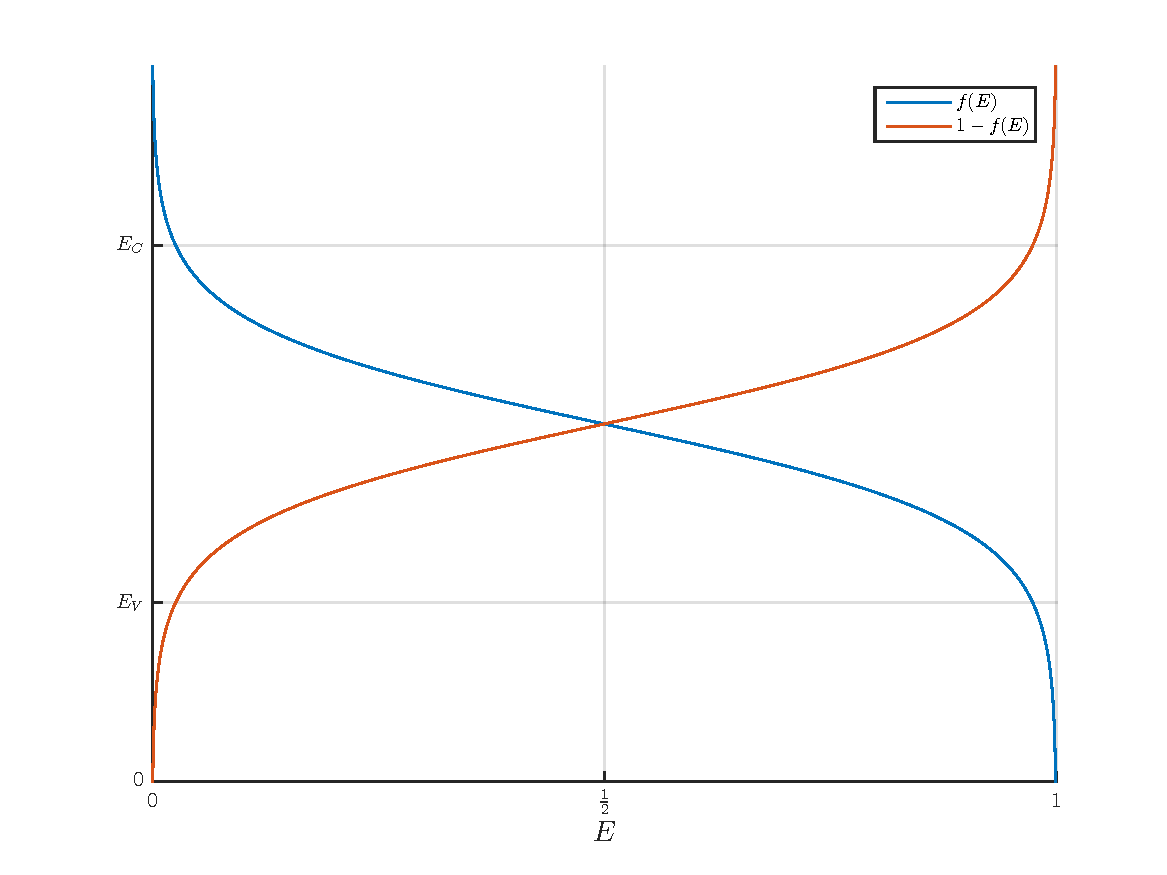
\includegraphics[width = 0.8\textwidth]{./Plots/fermi_function_vertical.pdf}
	\caption{Graph of $f(E)$ and $1 - f(E)$ with $E_C$ and $E_V$}
	\label{fig:Graph_of_$f(E)$_and_$1_-_f(E)$_with_$E_C$_and_$E_V$}
\end{figure}
The area bounded by $f(E)$ above $E_C$, in \cref{fig:Graph_of_$f(E)$_and_$1_-_f(E)$_with_$E_C$_and_$E_V$}, represents the number of electrons in the conduction band.
Similarly, the area bounded by $1 - f(E)$ below $E_V$, in \cref{fig:Graph_of_$f(E)$_and_$1_-_f(E)$_with_$E_C$_and_$E_V$}, represents the number of holes in the valence band.\\
The densities of states for electrons and holes are given by
\begin{align*}
	g_C(E) & = \frac{4 \pi}{h^3} \left( 2 {m_e}^* \right)^{\frac{3}{2}} (E - E_C)^{\frac{1}{2}} \\
	g_V(E) & = \frac{4 \pi}{h^3} \left( 2 {m_h}^* \right)^{\frac{3}{2}} (E_V - E)^{\frac{1}{2}}
\end{align*}
Therefore, substituting and solving,
\begin{align*}
	n & = \frac{2}{h^3} \left( 2 \pi {m_e}^* k T \right)^{\frac{3}{2}} e^{-\frac{E_C - E_F}{k T}} \\
	p & = \frac{2}{h^3} \left( 2 \pi {m_h}^* k T \right)^{\frac{3}{2}} e^{-\frac{E_F - E_V}{k T}}
\end{align*}
The constants
\begin{align*}
	N_C & = \frac{2}{h^3} \left( 2 \pi {m_e}^* k T \right)^{\frac{3}{2}} \\
	N_V & = \frac{2}{h^3} \left( 2 \pi {m_h}^* k T \right)^{\frac{3}{2}} \\
\end{align*}
are called the effective density of states in the conduction band and the valence band respectively.

\subsection{Intrinsic Semiconductor}

At $0 \kelvin$, all electrons are in the valence band.
Therefore, for all electrons to be below $E_F$, $E_F$ must be between $E_C$ and $E_V$.\\
As the material is an intrinsic semiconductor,
\begin{align*}
	n                                                                          & = p                                                               \\
	\therefore \left( {m_e}^* \right)^{\frac{3}{2}} e^{-\frac{E_C - E_F}{k T}} & = \left( {m_h}^* \right)^{\frac{3}{2}} e^{-\frac{E_F - E_V}{k T}} \\
	\therefore \left( \frac{{m_e}^*}{{m_h}^*} \right)^{\frac{3}{2}}            & = e^{-\frac{E_F - E_V}{k T}} e^{\frac{E_C - E_F}{k T}}            \\
                                                                                   & = e^{\frac{E_C + E_V - 2 E_F}{k T}}
\end{align*}
Assuming ${m_e}^* = {m_h}^*$,
\begin{align*}
	1              & = e^{\frac{E_C + E_V - 2 E_F}{k T}} \\
	\therefore E_F & = \frac{E_C + E_V}{2}               \\
	\therefore E_F & = E_i
\end{align*}
Realistically, ${m_e}^* > {m_h}^*$.
Therefore, $E_F$ is below $E_i$.
However, as the difference between the effective masses, and hence $E_F$ and $E_i$ is small,
\begin{align*}
	E_F & \approx E_i
\end{align*}
This can be used as a practical approximation.
\begin{figure}[h]
	\centering
	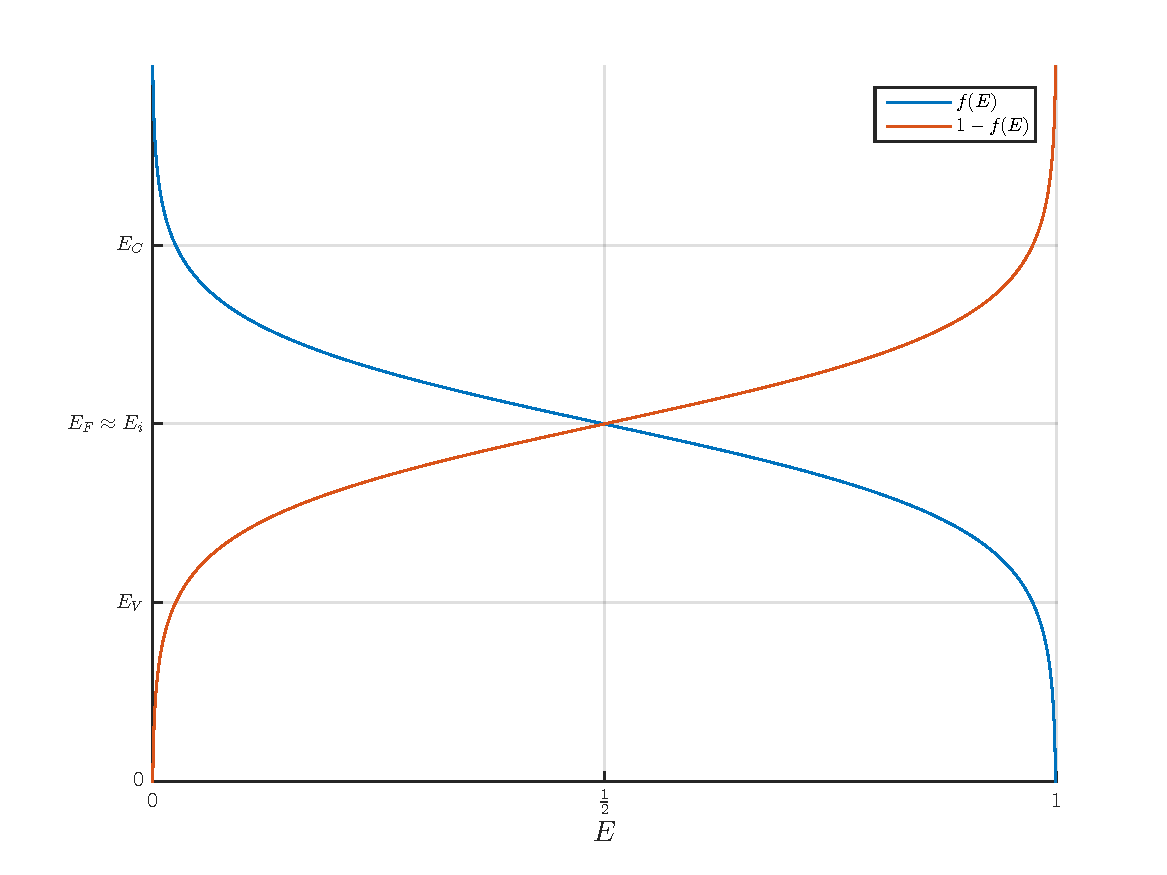
\includegraphics[width = 0.8\textwidth]{./Plots/fermi_function_for_intrinsic.pdf}
	\caption{Position of $E_F$ for an Intrinsic semiconductor}
	\label{fig:Position_of_$E_F$_for_an_Intrinsic_semiconductor}
\end{figure}

\subsection{N-type Semiconductor}

In a N-type semiconductor,
\begin{align*}
	n & > p
\end{align*}
As $0 \kelvin$, all electrons must be either at in the valence band, or at $E_d$.
Therefore, for all electrons to be below $E_F$, $E_F$ must be between $E_d$ and $E_C$.
Therefore, as $E_d$ is closer to $E_C$ than to $E_V$, $E_F$ is also closer to $E_C$ than to $E_V$.\\
The number of electrons in the conduction band is equal to the area under the curve of $f(E)$, to the right of $E_C$.
\begin{figure}[h]
	\centering
	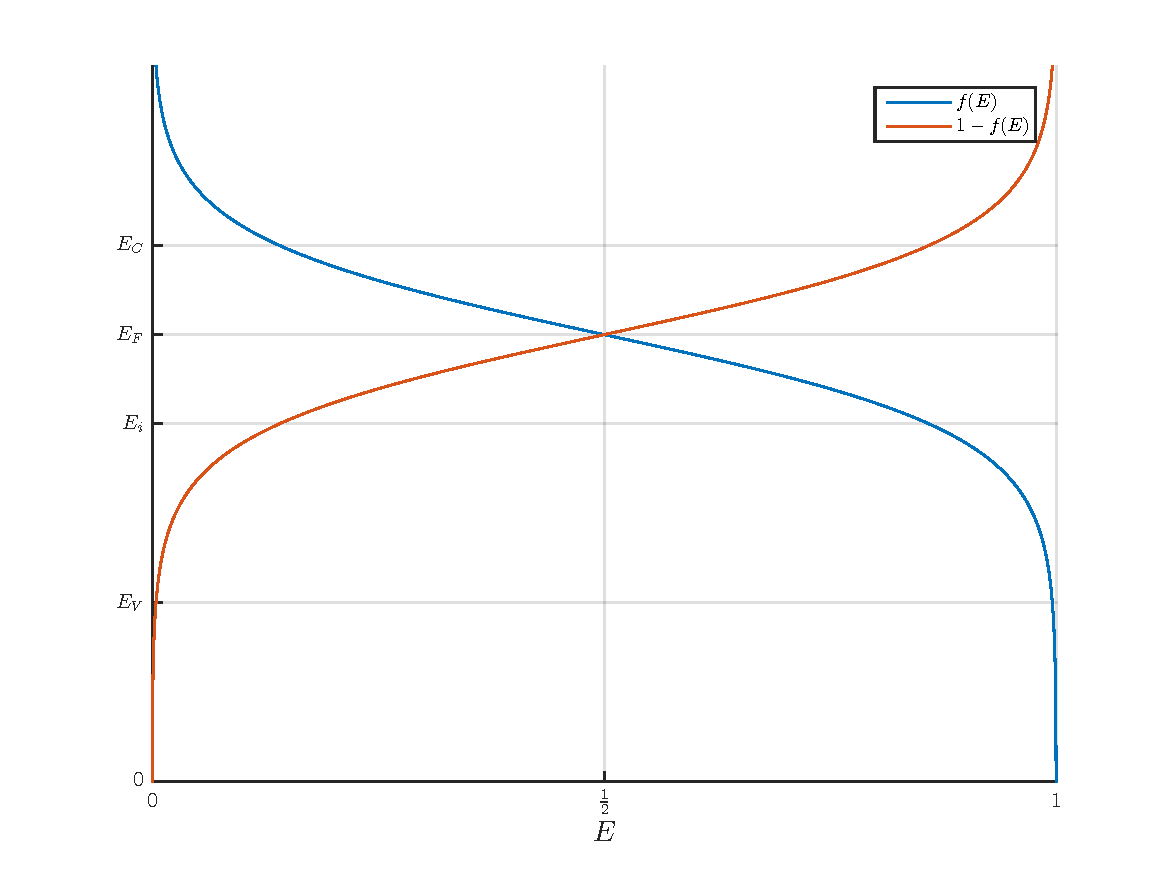
\includegraphics[width = 0.8\textwidth]{./Plots/fermi_function_for_N_type.pdf}
	\caption{Position of $E_F$ for an N-type semiconductor}
	\label{fig:Position_of_$E_F$_for_an_N-type_semiconductor}
\end{figure}

\subsection{P-type Semiconductor}

In a P-type semiconductor,
\begin{align*}
	p & > n
\end{align*}
As $0 \kelvin$, all electrons must be either at in the valence band, or at $E_a$.
Therefore, for all electrons to be below $E_F$, $E_F$ must be between $E_a$ and $E_C$.
Therefore, as $E_a$ is closer to $E_V$ than to $E_C$, $E_F$ is also closer to $E_V$ than to $E_C$.
\begin{figure}[h]
	\centering
	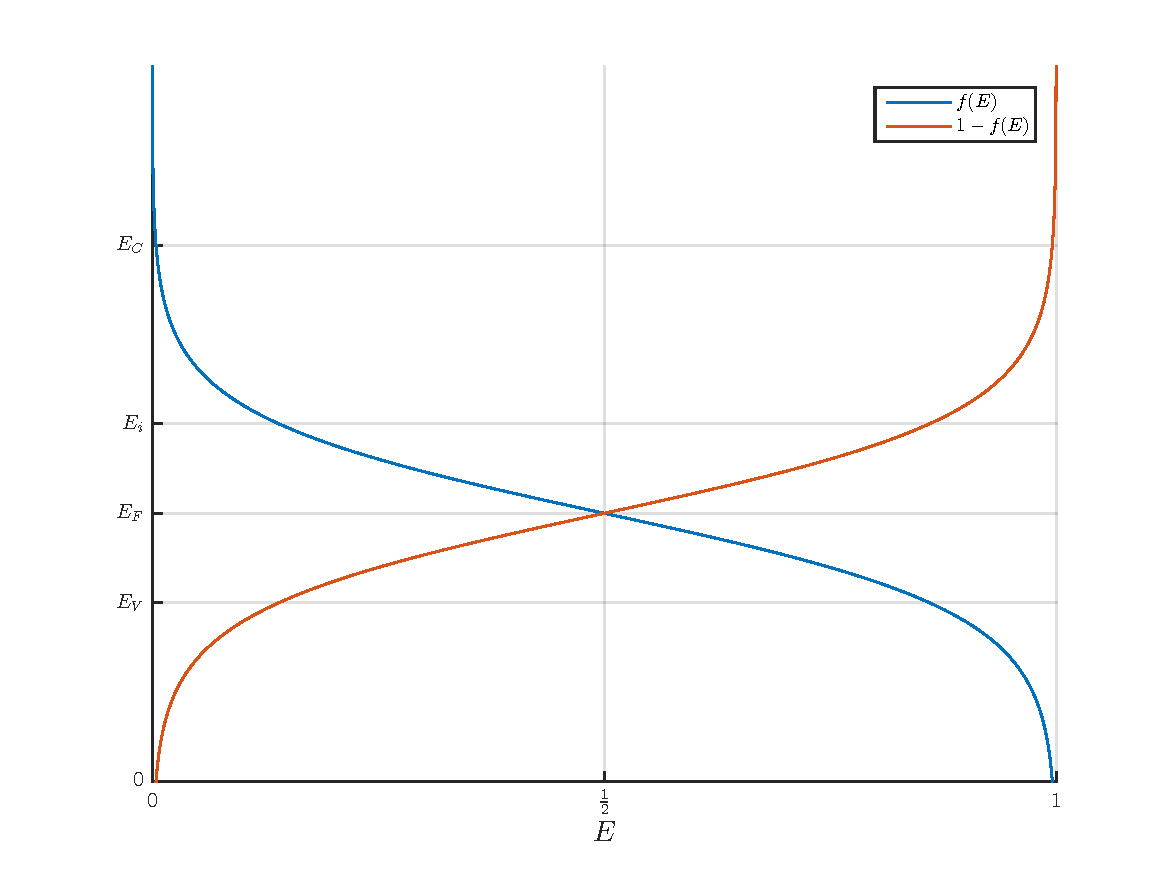
\includegraphics[width = 0.8\textwidth]{./Plots/fermi_function_for_P_type.pdf}
	\caption{Position of $E_F$ for an P-type semiconductor}
	\label{fig:Position_of_$E_F$_for_an_P-type_semiconductor}
\end{figure}

\section{Graphical Representation of Number of Electrons in the Conduction Band}

The number of allowed states in the conduction band is given by
\begin{align*}
	g_C(E) & = \frac{4 \pi}{h^3} \left( 2 {m_e}^* \right)^{\frac{3}{2}} (E - E_C)^{\frac{1}{2}} \\
               & \approx \sqrt{E - E_C}
\end{align*}
The probability of an energy state $E$ being occupied is given by
\begin{align*}
	f(E) & = \frac{1}{1 + e^{\frac{E - E_F}{k T}}}
\end{align*}
Therefore, the electron distribution in the conduction band is
\begin{align*}
	g_C(E) f(E) & = \sqrt{E - E_C} \frac{1}{1 + e^{\frac{E - E_F}{k T}}}
\end{align*}
Therefore, as $g_C(E)$ is zero for $E < E_C$, the graph of the electron distribution function is as in \cref{fig:Electron_distribution_function_in_the_conduction_band}.
\begin{figure}[h]
	\centering
	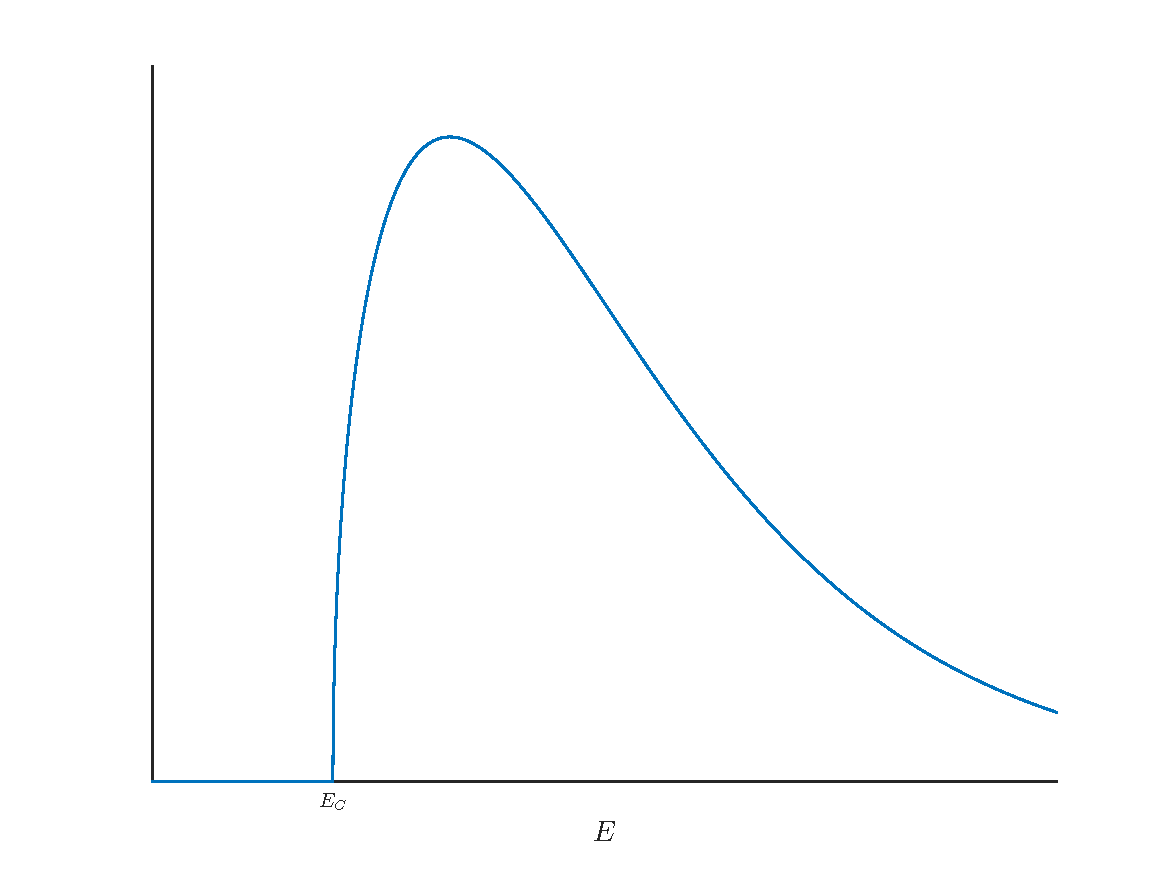
\includegraphics[width = 0.8\textwidth]{./Plots/electron_distribution_in_conduction_band.pdf}
	\caption{Electron distribution function in the conduction band}
	\label{fig:Electron_distribution_function_in_the_conduction_band}
\end{figure}

\section{Maxwell-Boltzmann Approximation}

The number of allowed states in the gap between the valence and conduction bands is zero.
Therefore, although the Fermi function is non zero in the energy gap, the number of electrons in the conduction band can be approximated as
\begin{align*}
	\frac{1}{1 + e^{\frac{E - E_F}{k T}}} & \approx e^{-\frac{E - E_F}{k T}}
\end{align*}
Therefore, integrating and solving,
\begin{align*}
	n & = N_C e^{\frac{E_C - E_F}{k T}}
\end{align*}
where $N_C$ is a constant which represents the effective density of states, and not a function of $E$.\\
Therefore, at equilibrium,
\begin{align*}
	n_0 & = N_C e^{-\frac{E_C - E_F}{k T}} \\
	p_0 & = N_V e^{-\frac{E_F - E_V}{k T}}
\end{align*}
Therefore,
\begin{align*}
	{n_i}^2        & = n_0 p_0                            \\
                       & = N_C N_V e^{-\frac{E_C - E_V}{k T}} \\
	\therefore n_i & = \sqrt{N_C N_V} e^{-\frac{E_{\text{gap}}}{2 k T}}
\end{align*}
Therefore,
\begin{align*}
	n & = N_C e^{-\frac{E_C - E_F}{k T}} \\
          & = N_C e^{-\frac{E_C - E_i}{k T}} e^{-\frac{E_i - E_F}{k T}}
\end{align*}
For an intrinsic material, i.e. when $E_F = E_i$,
\begin{align*}
	n & = n_i \\
\end{align*}
Therefore,
\begin{align*}
	n & = n_i e^{\frac{E_F - E_i}{k T}}
\end{align*}
Similarly,
\begin{align*}
	p & = n_i e^{\frac{E_i - E_F}{k T}}
\end{align*}
Therefore,
\begin{align*}
	E_F - E_i & = k T \ln\left( \frac{n}{n_i} \right) \\
	E_i - E_F & = k T \ln\left( \frac{p}{n_i} \right)
\end{align*}

\begin{question}
	Consider a sample of Si, doped with
	\begin{align*}
		N_D & = 10^{16} \si{\per\centi\metre\cubed}
	\end{align*}
	such that
	\begin{align*}
		E_C - E_D & = 0.05 \electronvolt
	\end{align*}
	\begin{enumerate}
		\item
			Draw $E_F$ as a function of $T$.
		\item
			How many dopants are ionized when $E_F = E_D$?
		\item
			Given
			\begin{align*}
				N_C & = 5 \times 10^{18} \si{\per\centi\metre\cubed}
			\end{align*}
			calculate the temperature when
			\begin{align*}
				E_F & = E_D
			\end{align*}
	\end{enumerate}
\end{question}

\begin{solution}
	\begin{enumerate}[leftmargin=*]
		\item
			Let the boundaries between the ionization and extrinsic regions and the extrinsic and intrinsic regions be $T_1$ and $T_2$ respectively.
			Therefore, for the ionization region, i.e. for $T < T_1$,
			\begin{align*}
				f(E < E_D) & = 1
			\end{align*}
			Therefore, $E_F$ is between $E_D$ and $E_C$.\\
			As the temperature increases, the some of the electrons which were previously at $E_D$ move to $E_C$.
			Therefore, the probability of electrons occupying the states at $E_D$ reduces, and that of $E_C$ increases.
			Therefore, the graph of $f(E)$ spreads out.
			Therefore, $E_F$ moves lower, and approaches $E_D$.\\
			Similarly, in the extrinsic region, $E_F$ is below $E_D$, and continues to move lower with increase in temperature.
			As the intrinsic carriers start ionizing, the rate of lowering of $E_F$ increases.\\
			In the intrinsic region,
			\begin{align*}
				E_F & = E_i
			\end{align*}
		\item
			\begin{align*}
				f(E_F)            & = \frac{1}{2} \\
				\therefore f(E_D) & = \frac{1}{2}
			\end{align*}
			Therefore, exactly half of the dopant states are occupied.
			Therefore, exactly half of the dopants are ionized.
		\item
			\begin{align*}
				n                                              & = N_C e^{-\frac{E_C - E_f}{k T}} \\
				\therefore \frac{N_D}{2}                       & = N_C e^{-\frac{E_C - E_D}{k T}} \\
				\therefore \ln\left( \frac{N_D}{2 N_C} \right) & = -\frac{E_C - E_D}{k T}         \\
				\therefore \ln\left( \frac{2 N_C}{N_D} \right) & = \frac{E_C - E_D}{k T}          \\
			\end{align*}
			Therefore,
			\begin{align*}
				T & = \frac{E_C - E_D}{k \ln\left( \frac{2 N_C}{N_D} \right)}                                                                                              \\
                                  & = \frac{0.05 \si{\electronvolt}}{\left( 8.6 \times 10^{-5} \si{\electronvolt\per\kelvin} \right) \ln\left( \frac{2.5 \times 10^{18}}{10^{16}} \right)} \\
                                  & = 85 \si{\kelvin}
			\end{align*}
	\end{enumerate}
\end{solution}

\begin{question}
	Consider a sample of Si at 300 \kelvin.
	The band diagram is as given.
	\begin{figure}[H]
		\centering
		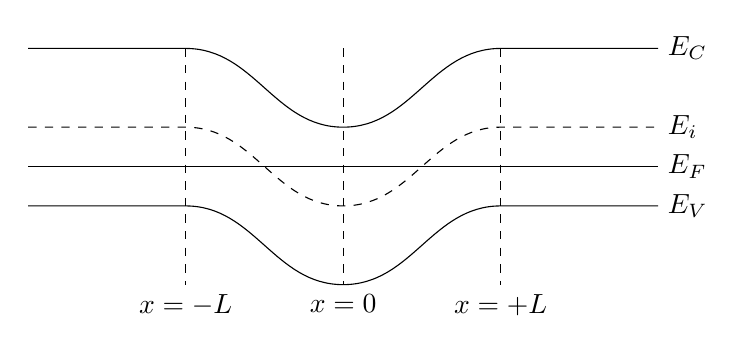
\begin{tikzpicture}
			\def\l{2};
			\def\L{3};
			\def\h{1};
			\def\eValence{0};
			\def\eIntrinsic{1};
			\def\eConduction{2};
			\def\eFermi{0.5};

			\begin{scope}[yshift = \eValence cm]
				\draw (-2*\l,0) to (-\l,0) to [out = 0, in = 180] (0,-\h) to [out = 0, in = 180] (\l,0) to (2*\l,0) node [right] {$E_V$};
			\end{scope}

			\begin{scope}[yshift = \eIntrinsic cm, dashed]
				\draw (-2*\l,0) to (-\l,0) to [out = 0, in = 180] (0,-\h) to [out = 0, in = 180] (\l,0) to (2*\l,0) node [right] {$E_i$};
			\end{scope}

			\begin{scope}[yshift = \eConduction cm]
				\draw (-2*\l,0) to (-\l,0) to [out = 0, in = 180] (0,-\h) to [out = 0, in = 180] (\l,0) to (2*\l,0) node [right] {$E_C$};
			\end{scope}

			\begin{scope}
				\draw (-2*\l,\eFermi) -- (2*\l,\eFermi) node [right] {$E_F$};
			\end{scope}
			
			\begin{scope}[dashed]
				\draw (-\l,\eConduction) -- (-\l,{\eValence - \h}) node [below] {$x = -L$};
				\draw (0,{\eConduction}) -- (0,{\eValence - \h}) node [below] {$x = 0$};
				\draw (\l,\eConduction) -- (\l,{\eValence - \h}) node [below] {$x = +L$};
			\end{scope}
		\end{tikzpicture}
	\end{figure}
	Assume that at $x = 0$,
	\begin{align*}
		E_F - E_i & = \frac{E_{\text{gap}}}{4}
	\end{align*}
	and at $x = \pm L$,
	\begin{align*}
		E_i - E_F & = \frac{E_{\text{gap}}}{4}
	\end{align*}
	\begin{enumerate}
		\item Sketch $V(x)$, the electrostatic potential in the sample.
		\item Sketch the electric field $\mathcal{E}(x)$.
		\item Identify the different regions.
		\item Sketch the concentrations of the electrons and the holes.
		\item Find the directions of the electron currents.
	\end{enumerate}
\end{question}

\begin{solution}
	\begin{enumerate}[leftmargin=*]
		\item
			\begin{align*}
				E & = -q V
			\end{align*}
			Therefore, the graph of of $V(x)$ is
			\begin{figure}[H]
				\centering
				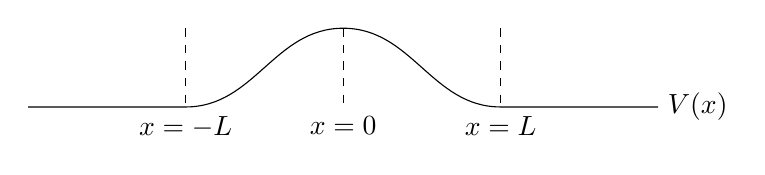
\begin{tikzpicture}
					\def\l{2};
					\def\L{3};
					\def\h{1};

					\draw (-2*\l,0) to (-\l,0) to [out = 0, in = 180] (0,\h) to [out = 0, in = 180] (\l,0) to (2*\l,0) node [right] {$V(x)$};

					\begin{scope}[dashed]
						\draw (-\l,\h) -- (-\l,0) node [below] {$x = -L$};
						\draw (0,\h) -- (0,0) node [below] {$x = 0$};
						\draw (\l,\h) -- (\l,0) node [below] {$x = L$};
					\end{scope}
				\end{tikzpicture}
			\end{figure}
		\item
			By Poisson's Equation,
			\begin{align*}
				\dod{V}{x} & = -\mathcal{E}
			\end{align*}
			Therefore, the graph of the field is of the form
			\begin{figure}[H]
				\centering
				\begin{tikzpicture}
					\def\l{2};
					\def\L{3};
					\def\h{1};

					\draw [rounded corners] (-2*\l,0) to (-\l,0) to [out = 0, in = 135] (-\l/2,-\h) to [out = 0, in = 180] (\l/2,\h) to [out = -45, in = 180] (\l,0) to (2*\l,0) node [right] {$V(x)$};

					\begin{scope}[dashed]
						\draw (-\l,\h) -- (-\l,0) node [below] {$x = -L$};
						\draw (0,\h) -- (0,0) node [below] {$x = 0$};
						\draw (\l,\h) -- (\l,0) node [below] {$x = L$};
					\end{scope}
				\end{tikzpicture}
			\end{figure}
		\item
			For $x < -L$, $E_F$ is below $E_i$.
			Therefore, the material is P-type.\\
			Therefore,
			\begin{align*}
				p & = n_i e^{\frac{E_i - E_f}{k T}}            \\
                                  & = 10^{10} e^{\frac{E_{\text{gap}}}{4 k T}} \\
                                  & = 3.92 \times 10^{14} \si{\per\centi\metre\cubed}
			\end{align*}
			Therefore,
			\begin{align*}
				n & = \frac{{n_i}^2}{p}                   \\
                                  & = \frac{10^{20}}{3.92 \times 10^{14}} \\
                                  & = 2.55 \times 10^5 \si{\per\centi\metre\cubed}
			\end{align*}
			~\\
			For $x = 0$, $E_F$ is above $E_i$.
			Therefore, the material is N-type.\\
			Therefore,
			\begin{align*}
				n & = n_i e^{\frac{E_i - E_f}{k T}}            \\
                                  & = 10^{10} e^{\frac{E_{\text{gap}}}{4 k T}} \\
                                  & = 3.92 \times 10^{14} \si{\per\centi\metre\cubed}
			\end{align*}
			Therefore,
			\begin{align*}
				p & = \frac{{n_i}^2}{n}                   \\
                                  & = \frac{10^{20}}{3.92 \times 10^{14}} \\
                                  & = 2.55 \times 10^5 \si{\per\centi\metre\cubed}
			\end{align*}
			~\\
			For $x < -L$, $E_F$ is below $E_i$.
			Therefore, the material is P-type.\\
			Therefore,
			\begin{align*}
				p & = n_i e^{\frac{E_i - E_f}{k T}}            \\
                                  & = 10^{10} e^{\frac{E_{\text{gap}}}{4 k T}} \\
                                  & = 3.92 \times 10^{14} \si{\per\centi\metre\cubed}
			\end{align*}
			Therefore,
			\begin{align*}
				n & = \frac{{n_i}^2}{p}                   \\
                                  & = \frac{10^{20}}{3.92 \times 10^{14}} \\
                                  & = 2.55 \times 10^5 \si{\per\centi\metre\cubed}
			\end{align*}
		\item
			~\\
			\begin{figure}[H]
				\centering
				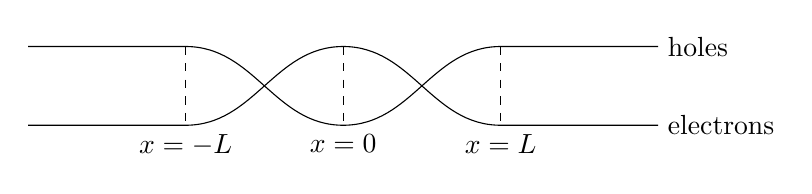
\begin{tikzpicture}
					\def\l{2};
					\def\L{3};
					\def\h{1};

					\draw (-2*\l,0) to (-\l,0) to [out = 0, in = 180] (0,\h) to [out = 0, in = 180] (\l,0) to (2*\l,0) node [right] {electrons};
					\draw [yshift = \h cm] (-2*\l,0) to (-\l,0) to [out = 0, in = 180] (0,-\h) to [out = 0, in = 180] (\l,0) to (2*\l,0) node [right] {holes};

					\begin{scope}[dashed]
						\draw (-\l,\h) -- (-\l,0) node [below] {$x = -L$};
						\draw (0,\h) -- (0,0) node [below] {$x = 0$};
						\draw (\l,\h) -- (\l,0) node [below] {$x = L$};
					\end{scope}
				\end{tikzpicture}
			\end{figure}
		\item
			The concentration of the electrons is higher at the centre that at the ends.
			Therefore, the electrons flow outwards.
			Therefore, the electron diffusion current is directed outwards.\\
			The electric field is directed leftwards for $x < 0$, and rightwards for $x > 0$.
			Therefore, the electron drift current is directed inwards.
	\end{enumerate}
\end{solution}

\section{Space Charge Neutrality}

For a material to be neutral, the total negative charges must be equal to the total positive charges.
Therefore,
\begin{align*}
	n_0 + {N_A}^- & = p_0 + {N_D}^-
\end{align*}
Also,
\begin{align*}
	n_0     & = N_C e^{-\frac{E_C - E_F}{k T}} \\
	p_0     & = N_V e^{-\frac{E_F - E_V}{k T}} \\
	{N_A}^- & = N_A f(E_A)                     \\
	{N_D}^+ & = N_D \left( 1 - f(E_A) \right)
\end{align*}
Therefore,
\begin{align*}
	N_C e^{-\frac{E_C - E_F}{k T}} + N_A f(E_A) & = N_V e^{-\frac{E_F - E_V}{k T}} + N_D \left( 1 - f(E_D) \right)
\end{align*}

\clearpage
\part{PN Junctions}

\section{Step Junction}

\begin{definition}[Electron affinity]
	The electron affinity for a semiconductor is defined to be
	\begin{align*}
		q \chi & = E_{\text{vac}} - E_C
	\end{align*}
	where $E_{\text{vac}}$ is the energy of a free particle.
	The electron affinity is material dependent.\\
\end{definition}

\begin{definition}[Semiconductor work function]
	The semiconductor work function is defined to be
	\begin{align*}
		q \Phi_S & = E_{\text{vac}} - E_F
	\end{align*}
	The semiconductor work function is doping dependent.
\end{definition}

Consider a P-type semiconductor with $p = N_A$ and a N-type semiconductor with $n = N_D$.\\
Let the two be placed separately.\\
Let $E_{F_p}$ and $E_{F_n}$ be the Fermi levels for the P-type and the N-type semiconductors respectively.\\
Therefore,
\begin{align*}
	q \chi       & = E_{\text{vac}} - E_C     \\
	q \Phi_{S_p} & = E_{\text{vac}} - E_{F_p} \\
	q \Phi_{S_n} & = E_{\text{vac}} - E_{F_n}
\end{align*}
Let these semiconductors be brought into contact as in \cref{fig:Structure_of_Step_PN_Junction} and allowed to reach equilibrium.
\begin{figure}[h]
	\centering
	\begin{tikzpicture}
		\def\l{2};
		\def\h{1};

		\draw (-\l,-\h/2) rectangle (0,\h/2);
		\draw (-,-\h/2) rectangle (\l,\h/2);

		\node at (-\l/2,0) {P-type};
		\node at (\l/2,0) {N-type};
	\end{tikzpicture}
	\caption{Structure of Step PN Junction}
	\label{fig:Structure_of_Step_PN_Junction}
\end{figure}
At equilibrium, the Fermi levels must match up, and $E_F$ must be constant.\\
~\\
The carrier concentrations in the junction are as in \cref{fig:Carrier_Concentrations_in_Step_PN_Junction}.
\begin{figure}[h]
	\centering
	\begin{tikzpicture}
		\def\xMIN{-4};
		\def\xMAX{4};
		\def\yMIN{-4};
		\def\yMAX{4};
		\def\NA{-2};
		\def\ND{2};

		\begin{scope}[stealth-stealth]
			\draw (\xMIN,0) -- (\xMAX,0) node [right] {$x$};
			\draw (0,\yMIN) -- (0,\yMAX);
		\end{scope}

		\begin{scope}
			\draw (\xMIN,\NA) node [left] {$N_A$} -- (0,\NA);
			\draw (0,\ND) -- (\xMAX,\ND) node [right] {$N_D$};
			\node [above] at (\xMIN/2,\yMAX) {P-type};
			\node [above] at (\xMAX/2,\yMAX) {N-type};
		\end{scope}
	\end{tikzpicture}
	\caption{Carrier Concentrations in Step PN Junction}
	\label{fig:Carrier_Concentrations_in_Step_PN_Junction}
\end{figure}
Therefore, the carriers diffuse from regions of higher concentration to regions of lower concentrations, i.e., the electrons diffuse from the N-type region to the P-type region, and the holes diffuse from the P-type region to the N-type region.\\
This diffusion occurs in a region closer to the junction, and not in the regions near the ends.
This region is called the depletion region.\\
As these mobile carriers diffuse, they leave behind the ionized dopants, which are fixed charges.
This causes an internal electric field $\mathcal{E}$ in the depletion region, directed from the N-type region to the P-type region.
This generated electric field repels the diffusing carriers.
Therefore, the diffusion is stopped.
The width of the depletion region when the diffusion stops is denoted by $W$ or $W_d$.\\
The width of the depletion region on the P-type side is denoted by $x_p$, and that on the N-type side is denoted by $x_n$.
~\\
The currents generated due to the drifting charge carriers are opposite in direction to the currents generated due to the diffusing charge carriers.
Therefore, the net current in the PN junction is zero.\\
\end{document}
